\section{Protocolo ARP}
\subsection*{Selecione um host (PC, servidor) de um departamento à sua escolha. Neste host inicie a
captura de tráfego com o Wireshark do CORE. A partir desse host efectue pings para dois
hosts localizados na rede do outro departamento. Pare a captura de tráfego no
Wireshark e localize o tráfego ARP, usando o filtro arp.}

\begin{figure} [h]
    \centering
    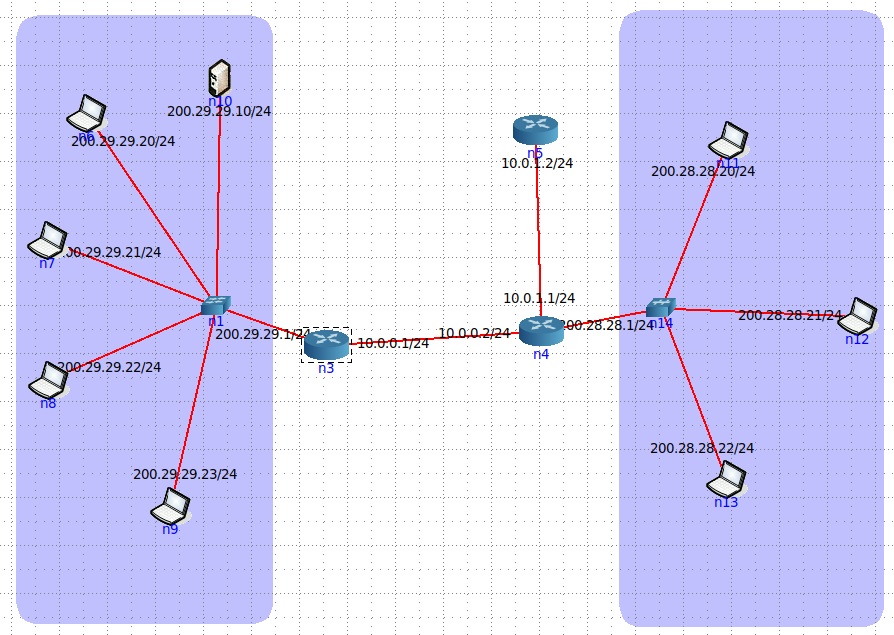
\includegraphics[width=0.8\linewidth]{images/ligacoes-routers.png}
    \caption{Rede}
    \label{fig:enter-label}
\end{figure}

\subsection{Abra uma consola no host onde efetou o ping. Observe o conteúdo da tabela ARP com o comando arp.}

\begin{figure} [h]
    \centering
    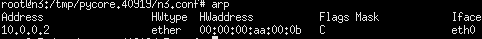
\includegraphics[width=0.8\linewidth]{images/dois-pings-tabela-arp.png}
    \caption{Enter Caption}
    \label{fig:enter-label}
\end{figure}

\subsubsection{Com a ajuda do manual arp (man arp), interprete sucintamente o significado de cada uma das colunas da tabela.}

\textbf{Address}: O endereço IP associado ao endereço MAC.

\textbf{HWtype}: O tipo de hardware, que é "ether" neste caso, indicando Ethernet.

\textbf{HWaddress}: O endereço MAC associado ao endereço IP.

\textbf{Flags}: As bandeiras indicam o estado da entrada na tabela. "C" significa que a entrada está completa, ou seja, o mapeamento IP-MAC é conhecido e válido.

\textbf{Mask}: Se estiver preenchido, indica uma máscara de sub-rede associada ao endereço IP.

\textbf{Iface}: A interface de rede à qual o endereço MAC está associado.\newline

Neste caso, com base na tabela ARP, existe apenas uma entrada:

\textbf{Endereço IP 10.0.0.2} está associado ao \textbf{endereço MAC 00:00:00:aa:00:0b}. A entrada na tabela ARP está marcada como completa (C) e associada à interface \textbf{eth0}.

Essa entrada significa que o endereço IP 10.0.0.2 está associado ao endereço MAC 00:00:00:aa:00:0b e que essa associação é conhecida e válida. Portanto, o sistema já possui essa informação na tabela ARP e não precisa fazer solicitações ARP adicionais para esse endereço, pois já tem o mapeamento IP-MAC correspondente.

\subsubsection{Indique, justificando, qual o equipamento da rede em questão que poderá apresentar a maior tabela ARP em termos de número de entradas.}

Na rede, o equipamento que provavelente apresenta um maior número de entradas na tabela ARP será, provavelmente, o router n3, uma vez que apresenta 6 ligações, ao invés do n4 que apresenta 5 ligações.

\subsubsection{Realize as operações necessárias para completar a tabela ARP identificada na alínea anterior. Indique como procedeu e apresente essa tabela completa.}

Para chegar a esta tabela ARP, é necessário dar \textit{ping} a todos os dispositivos ligados ao router n3 pelo terminal e, de seguida, é deve abrir outro terminal pelo router n3 e abrir a tabela arp, chegando a um resultado semelhante ao aqui mostrado.

\begin{figure} [h]
    \centering
    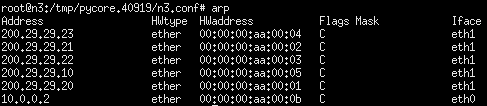
\includegraphics[width=0.8\linewidth]{images/tabela-arp-n3.png}
    \caption{Tabela ARP do router n3}
    \label{fig:enter-label}
\end{figure}

\subsection{Qual é o valor hexadecimal dos endereços origem e destino na trama Ethernet que contém a mensagem com o pedido ARP (ARP Request)? Como interpreta e justifica o endereço destino usado?}

\begin{figure} [h]
    \centering
    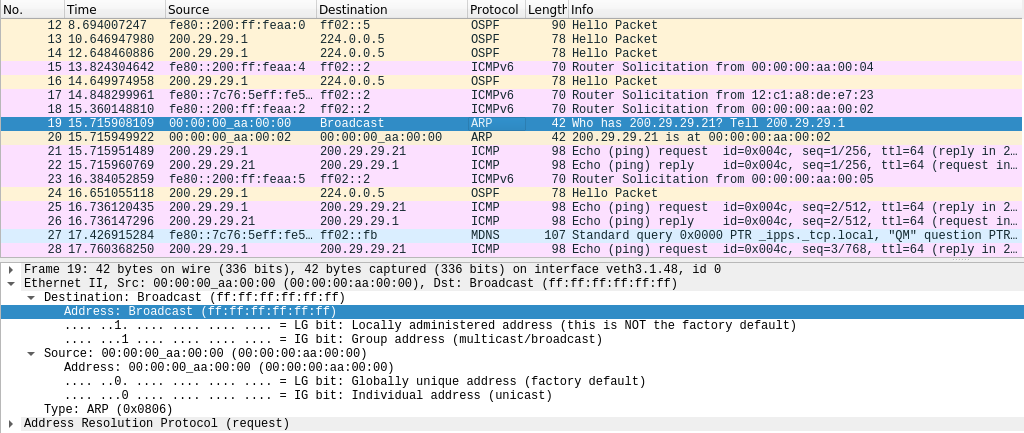
\includegraphics[width=0.8\linewidth]{images/arp-request-1.png}
    \caption{ARP Request}
    \label{fig:enter-label}
\end{figure}

O endereço de origem na trama Ethernet é 00:00:00:aa:00:00 e o endereço do destino é ff:ff:ff:ff:ff:ff. O endereço de Destino é um endereço de broadcast. Isto significa que a trama ARP está a ser enviada para todos os dispositivos na rede local para que o dispositivo de destino a reconheça. 

\subsection{Qual o valor hexadecimal no campo Tipo da trama Ethernet? O que indica?}


\begin{figure} [h]
    \centering
    
\includegraphics[width=0.5\linewidth]{images/tipo-arp-request.png}
    \caption{Enter Caption}
    \label{fig:enter-label}
\end{figure}

O valor hexadecimal no campo Tipo da trama Ethernet indica o tipo de dados que a trama contém. No caso de uma trama ARP, esse valor é 0x0806, que representa o protocolo ARP, como mostra a print tirada do wireshark.

\subsection{Observando a mensagem ARP, como pode saber que se trata efetivamente de um pedido ARP? Identifique o tipo de endereços contidos na mensagem ARP.}

É possível saber que se trata de um pedido ARP se observarmos o valor do campo "Opcode" (código de operação) na mensagem ARP. O valor 1 neste campo indica uma solicitação ARP. Os tipos de endereços contidos na mensagem ARP são o endereço IP e o endereço MAC.

\subsection{Explicite, em linguagem comum, que tipo de pedido ou pergunta é feita pelo host de origem à rede?}

O host de origem faz uma pergunta à rede, perguntando "Quem possui o endereço IP X?". Nesse caso, o host deseja mapear um endereço IP para um endereço MAC correspondente.

O host de origem pergunta à rede "Quem é possui este endereço IP?". Neste caso, o host quer mapear um endereço IP para um endereço MAC.

\subsection{Localize a mensagem ARP que é a resposta ao pedido ARP efetuado.}

\begin{figure} [h]
    \centering
    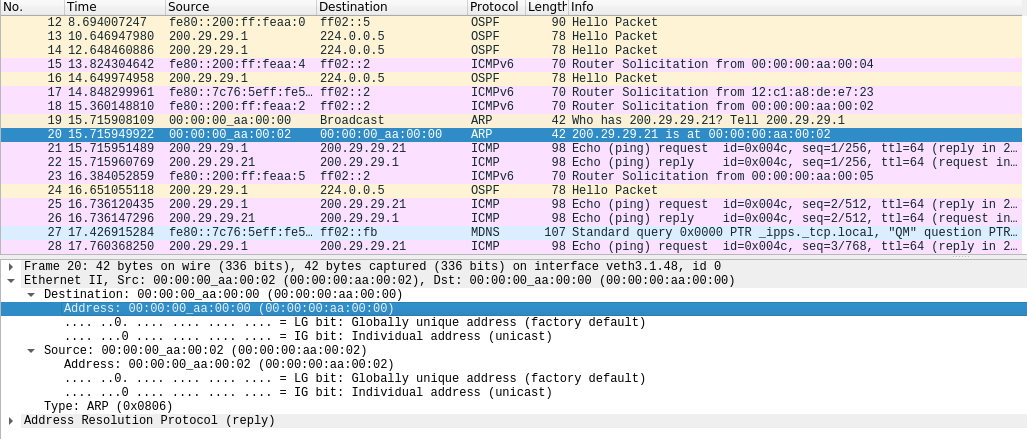
\includegraphics[width=0.8\linewidth]{images/resposta-arp-request.png}
    \caption{Mensagem ARP a responder ao pedido ARP}
    \label{fig:enter-label}
\end{figure}

A mensagem ARP em resposta ao pedido ARP está logo a seguir, como é possível ver no \textit{printscreen}.

\subsubsection{Qual o valor do campo ARP opcode? O que especifica?}

O valor do campo ARP opcode é 2, como é possível ver no \textit{printscreen} do pacote capturado pelo wireshark. Isto significa que é uma resposta ARP.

\begin{figure} [h]
    \centering
    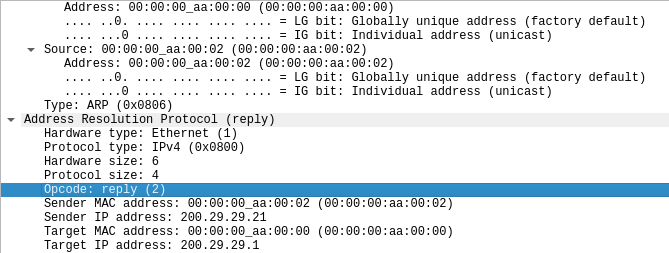
\includegraphics[width=0.8\linewidth]{images/opcode-arp-reply.png}
    \caption{ARP Opcode}
    \label{fig:enter-label}
\end{figure}

\subsubsection{Em que posição da mensagem ARP está a resposta ao pedido ARP?}

A resposta ao pedido ARP está na posição após o cabeçalho ARP (28 bytes).

\subsubsection{Justifique o modo de comunicação (unicast vs. broadcast) usado no envio da resposta ARP (ARP Reply).}

O ARP Request é enviado em \textbf{modo broadcast}, pois o host não sabe de quem é o endereço IP e precisa de perguntar a todos os dispositivos ligados quem é. A resposta ARP (ARP Reply) é enviada em \textbf{modo unicast}. Isso significa que a resposta é direcionada especificamente para o host que fez a pergunta ARP, uma vez que o dispositivo não tem necessidade de informar todos que é ele e precisa apenas de informar o host.

\subsection{Verifique se o ping feito ao segundo PC originou pacotes ARP e justifique a situação observada.}

O segundo ping feito também originou pacotes, como é possível ver no printscreen do wireshark.

\begin{figure} [h]
    \centering
    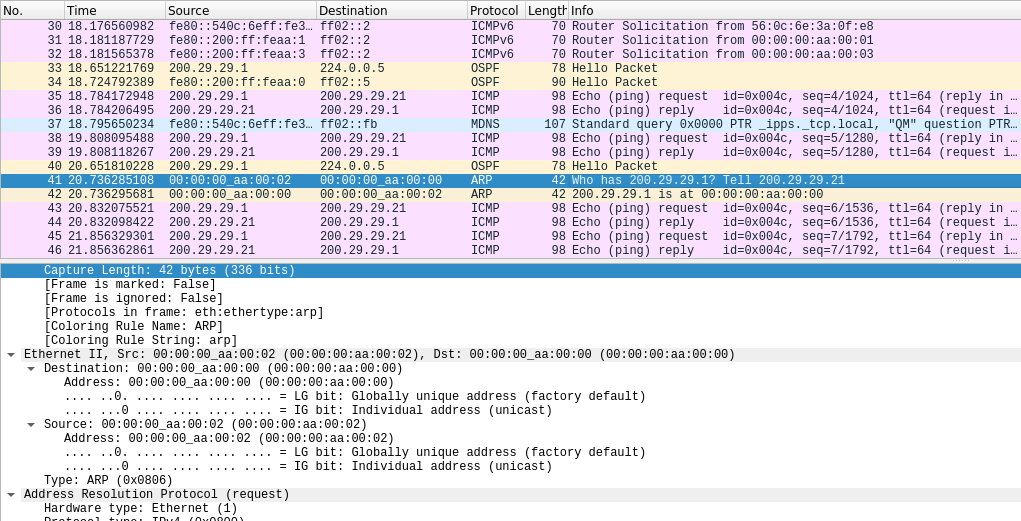
\includegraphics[width=0.8\linewidth]{images/segundo-ping-arp.png}
    \caption{Enter Caption}
    \label{fig:enter-label}
\end{figure}

\subsection{Identifique na mensagem ARP os campos que permitem definir o tipo e o tamanho dos endereços das camadas de rede e de ligação lógica que se pretendem mapear. Justifique os valores apresentados nesses campos.}

Os campos que permitem definir o tipo e o tamanho dos endereços das camadas de rede e de ligação lógica na mensagem ARP são:

\begin{itemize}
  \item \textbf{Tipo de Hardware}: Indica o tipo de hardware (geralmente Ethernet) e seu tamanho (6 bytes).
  \item \textbf{Tipo de Protocolo}: Indica o tipo de protocolo de rede (geralmente IPv4) e seu tamanho (4 bytes).
\end{itemize}
